
\documentclass{beamer}
\usepackage[utf8]{inputenc}
\usetheme{Warsaw}
\usecolortheme{seahorse}
\usepackage{listings}
\usepackage{color}
\usepackage{graphicx}

\definecolor{airforceblue}{rgb}{0.36, 0.54, 0.66}
\definecolor{darkWhite}{rgb}{0.94,0.94,0.94}
\newcommand{\TextSoulign}[3]{\emph{\textcolor{#1}{\underline{#2\textcolor{black}{#3}}}}}

\lstset{
backgroundcolor={darkWhite}
}


\title{Package Coberny}
\author{A.Bernard, F.Chery, O.Côme} \institute{
\includegraphics[scale=0.05]{logo.jpg} \newline Faculté des sciences de Montpellier}
\date{13 Décembre 2021}
\logo{
\includegraphics[scale=0.01]{logo_raccoon.png}}

\begin{document}
\begin{frame}
\titlepage
\end{frame}
\begin{frame}
\frametitle{Sommaire}
\tableofcontents
\end{frame}
\section{Introduction}
\subsection{Création de la base de données}

\begin{frame}[fragile]{Création de la base de données}
\TextSoulign{airforceblue}{Dataframe intermédiaire} : \newline
\begin{itemize}
\item Pour créer le data nous avons utilisé $\textbf{pandas}$ pour sélectionner uniquement les sorties d'autoroute concernées par le projet et enlever les portions gratuites.
\item Nous avons utilisé $\textbf{pyproj}$ pour transformer les coordonnées L93 en WGS84. Nous avons donc obtenu à la suite un dataframe avec les noms des autoroutes, les noms des péages et les coordonnées GPS.
\end{itemize}
\end{frame}


\begin{frame}[fragile]{Création de la base de données}
\begin{block}{Dataframe des prix}
Nous avons simplement reporté le fichier que nous avions en format $\textit{.csv}$ pour l'utiliser avec $\textbf{pandas}$ et choisir les péages voulus. Puis nous avons renommé les colonnes pour être cohérent avec les autres dataframe.
\end{block}
\begin{block}{Dataframe des distances}
Nous avons utilisé $\textbf{requests}$ et $\textbf{json}$ pour faire des requêtes de distance entre chaque coordonnées du dataframe créé précédemment. Ces packages utilisent les données de $\textbf{openstreetmap}$.
\end{block}
\end{frame}



\subsection{Présentation du package Coberny}

\begin{frame}[fragile]{Présentation du package Coberny}
\begin{block}{Installer Coberny}
pip install git+https://github.com/ABernard27/PROJET-groupe-3
\end{block}
Ce package permet de réaliser 3 actions primaires : \newline
\begin{itemize}
\item Réaliser une carte intéractive d'un trajet sur l'autoroute en affichant les noms des stations, le prix entre deux stations et le temps en kilomètres.
\item Afficher la distribution des prix entre deux sorties
\item Déterminer, en fonction du nombre de sorties acceptées, le trajet le moins coûteux
\end{itemize}
\end{frame}



\section{Carte intéractive}
\subsection{Création de la carte}

\begin{frame}[fragile]{Création de la carte}

La carte repose sur 3 packages essentiels : $\textbf{openrouteservice}$, $\textbf{json}$ et $\textbf{folium}$. Il y a une petite manipulation en plus pour exécuter cette fonction : créer une clé API sur $\textit{openrouteservice.org}$. \newline
\pause

Le code créé exécute des requêtes avec les points de coordonnées entrés pour relier tous ses points. L'API de direction renvoie des polylignes codés (série de coordonnées sous la forme d'une seule chaîne), à l'aide de
$\textit{convert.decode\_polyline}$ on peut les décoder. \newline
\pause

Ensuite $\textit{folium.GeoJson(decoded).add\_to(m)}$ ajoute à la carte les points reliés. $\textit{summary}$ permet de récupérer les distances dans le fichier json pour les afficher. Enfin, $\textit{folium.Marker}$ permet d'ajouter les marqueurs.
\end{frame}

\subsection{Utilisation}
\begin{frame}[fragile]{Utilisation}
Pour utiliser cette fonction les dataframe doivent être de la forme suivante : (extrait des tableaux) \newline
\only<1>{
\begin{center}
\begin{tabular}{|*{4}{c|}}
\hline
&MONTPELLIER&SETE&AGDE \\
\hline
0&0.0&1.6&3.6\\
\hline
1&1.6&0.0&1.9 \\
\hline
2&3.6&1.9&0.0\\
\hline
\end{tabular} \newline
Extrait tableau des prix
\end{center}}
\only<2>{
\begin{center}
\begin{tabular}{|*{4}{c|}}
\hline
&MONTPELLIER&SETE&AGDE \\
\hline
MONTPELLIER&0.0&17.0&41.0\\
\hline
SETE&17.0&0.0&26.0 \\
\hline
AGDE&41.0&26.0&0.0\\
\hline
\end{tabular} \newline
Extrait tableau des distances
\end{center}}
\end{frame}

\subsection{Exemple}
\begin{frame}[fragile]{Exemple}
Par exemple our utiliser la fonction carte il suffit d'importer $\textbf{Coberny}$ puis de taper la commande suivante :
\begin{block}{Exemple d'utilisation}
Coberny.carte(np.column$\_$stack([data['x'],data['y']]), data[' Nom gare' ], 'Key', prix)
\end{block}
\pause

Ici data est un dataframe contenant les noms des péages ainsi que leur coordonnée (longitude, latitude), Key est la clé openrouteservice, et prix est le dataframe contenant les prix entre toutes les sections. \newline
\pause

Après avoir exécuter ce code nous obtenons la carte suivante où l'on peut cliquer sur les marqueurs et les portions de route :
\end{frame}

\begin{frame}[fragile]{Exemple}
\begin{center}
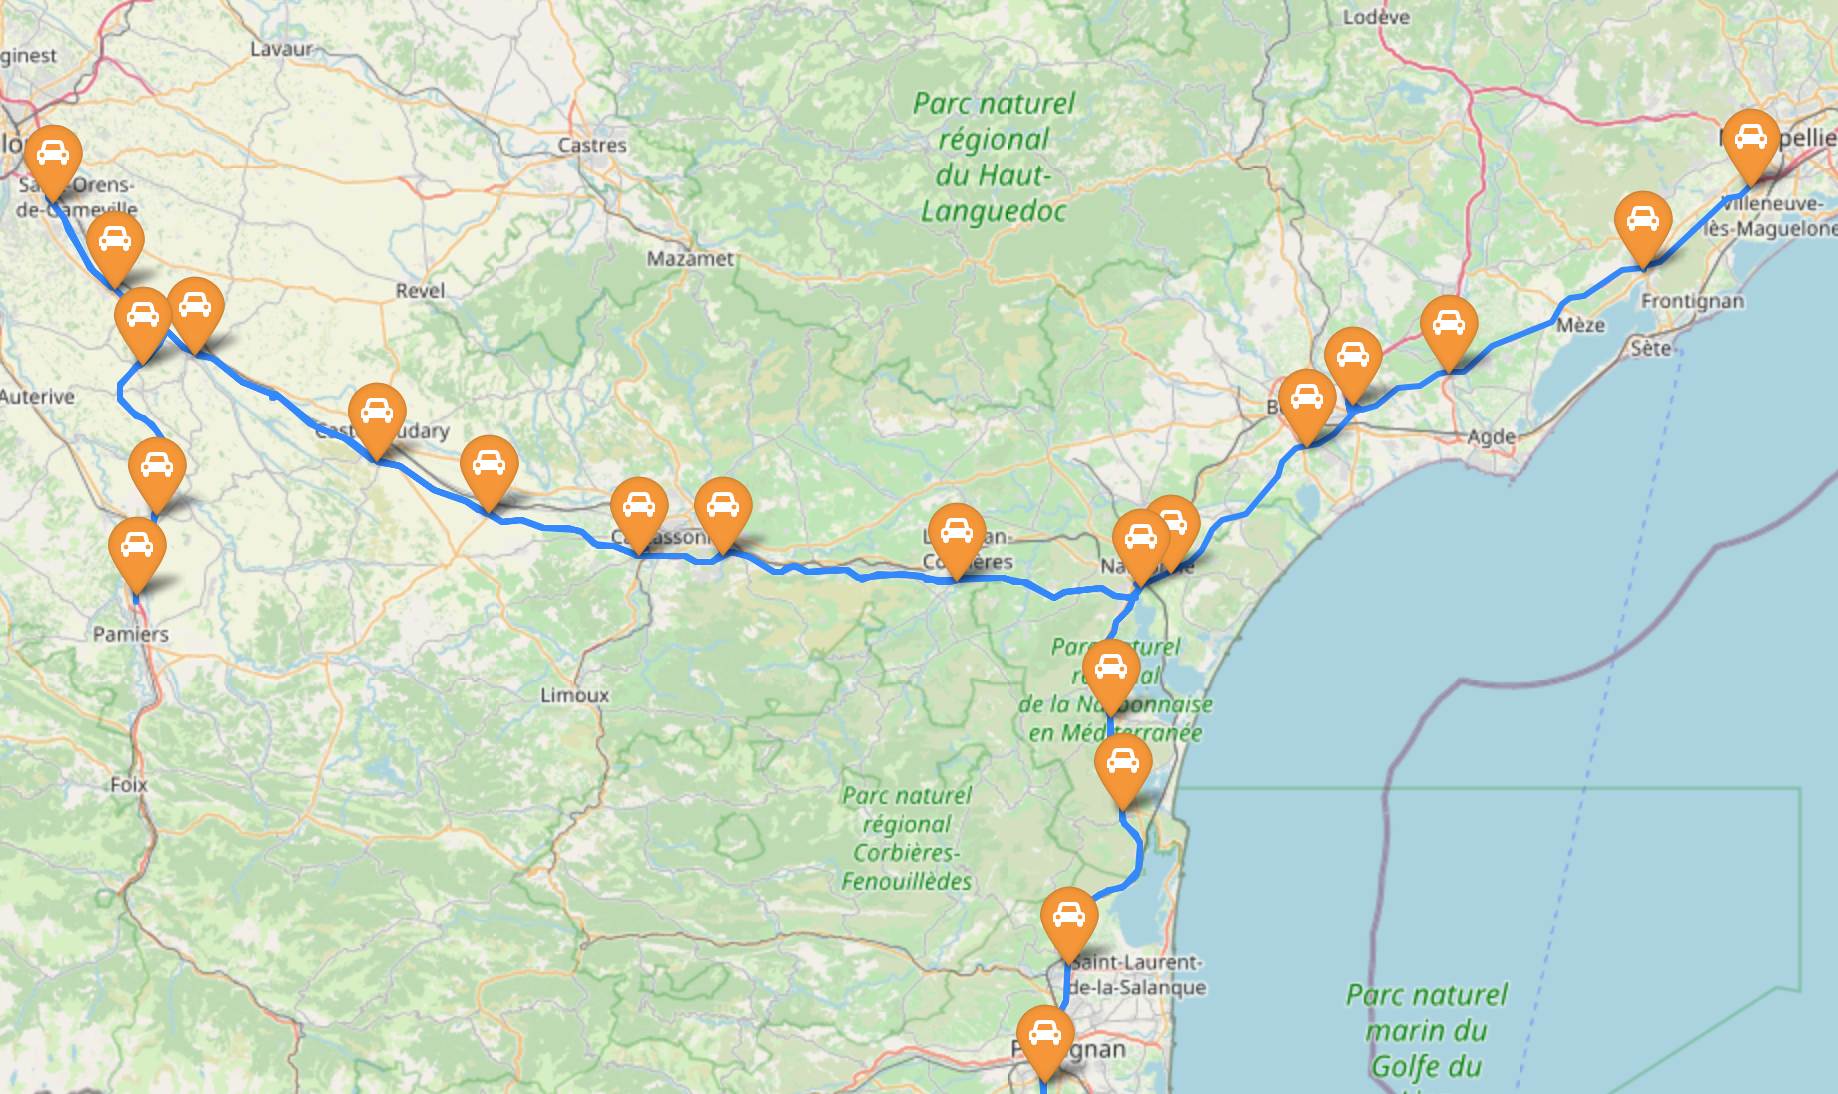
\includegraphics[scale=0.3]{carte.png}
\end{center}
\end{frame}

\section{Distribution des prix}
\subsection{Création du code}

\begin{frame}[fragile]{Code}
\begin{block}{Structute de la classe $\textbf{Distribution}$ }
\end{block}
\begin{itemize}
\item Une fonction $\textbf{Graph}$ qui contient deux définitions, et qui permet de visualiser le graphe du trajet. 
\pause
\item Définiton du Kernel Density Estimation : l’estimation par noyau est une méthode d’estimation de la densité de probabilité d’une variable aléatoire. 
\pause
\item Définition du Diagramme en bâton : représentation graphique de données à caractères discrets.
\pause
\item Le graphe du trajet avec le package $\textbf{networkx}$.
\end{itemize}
\pause
Nous avons utilisé la fonction $\textbf{interact}$ du package $\textbf{ipywidget}$, afin de tracer le KDE et le diagramme avec des widgets intéractifs.
\end{frame}

\begin{frame}[fragile]{Code}
Pour créer ces deux fonctions, nous avons eu besoin d'étapes intermediaires : 
\begin{itemize}
\item Récupération du trajet entre l'entrée et la sortie avec $\textbf{networkx et les graphes}$.
\item Construction du vecteur des prix au kilomètre par portion d'autoroute.
\end{itemize}
\pause
De plus, pour le bon fonctionnement du package nous avons créer une fonction  $\textbf{indice}$.

\end{frame}

\subsection{Utilisation}

\begin{frame}[fragile]{Utilisation}
Pour l'utilisation de cette classe, il nous faudra des dataframes de la même forme que pour la carte interactive. \newline
\pause
Avec la structure de classe, la commande de code est à utiliser sous cette forme là :
\pause
\begin{block}{Exemple d'utilisation:}
Coberny.distribution(dataframe distances, dataframe prix).Graph()
\end{block}

\end{frame}

\subsection{Exemple d'utilisation}
\begin{frame}[fragile]{Exemple d'utilisation}
\begin{block}{Exemple d'utilisation avec nos dataframes :}
Coberny.distribution(Distance, Prix).Graph()
\end{block}

Lors de l'excution de ce code, nous obtenons :  
\begin{figure}[!h]
    \centering
    \begin{subfigure}{}
        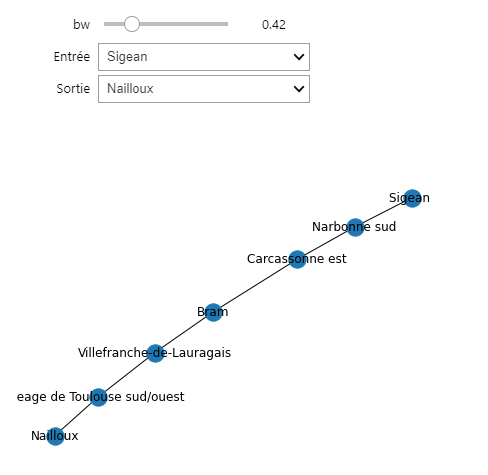
\includegraphics[width=5cm]{plot1.png}
    \end{subfigure}
    \begin{subfigure}
        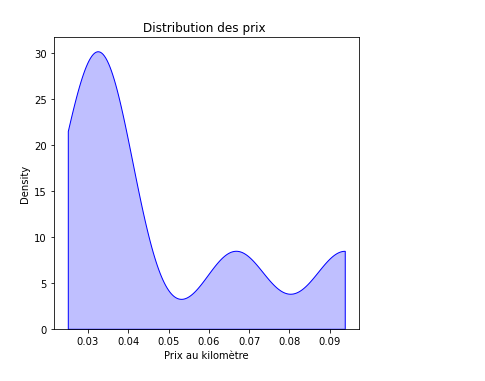
\includegraphics[width=5cm]{plot2.png}
    \end{subfigure}
\end{figure}
\end{frame}

\begin{frame}
\centerline{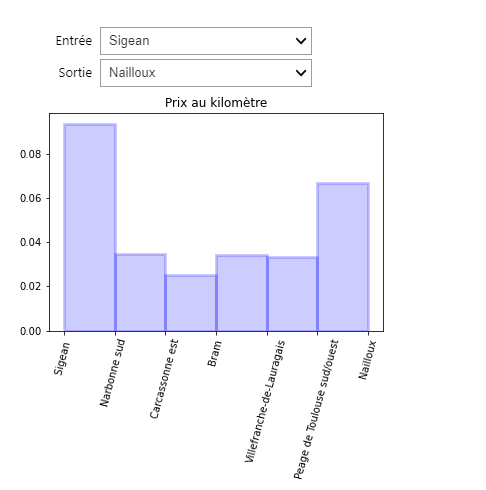
\includegraphics[width=8cm]{plot3.png}}

\end{frame}

\section{Minimisation coût du trajet}
\begin{frame}{Minimisation coût du trajet}
		\begin{block}{\scriptsize L'algorithme}
			\scriptsize
			L'algorithme permettant de déterminer le trajet le moins couteux en fonction du nombre de sorties acceptées repose sur 3 packages essentiels:
			\begin{itemize}
				\item \textbf{pandas:} Librairie utile afin de manipuler et d'analyser les données.
				\item \textbf{NetworkX:} Librairie pour le traitement de graphs.
				\item \textbf{itertools:} Module proposant un grand nombre d'itérateurs.
			\end{itemize}
			\vspace{3mm}
			L'algorithme possède deux fonctions principales:
			\begin{itemize}
				\item \textbf{FindBestPathForPrice} qui renvoie un couple contenant:
				\begin{itemize}
					\scriptsize
					\item La liste des péages par lesquelles il faudra passer pour payer le moins cher (il s'agit du trajet optimal).
					\item Le prix du trajet optimal.
				\end{itemize}
				\item \textbf{CreateGraphOfBestPathForPrice} qui trace le graph du trajet optimal.
				\begin{itemize}
					\scriptsize
					\item La ville de départ et celle d'arrivée sont coloriées en bleu.
					\item Les sorties intermédiaires sont coloriées en oranges.
				\end{itemize}
			\end{itemize}
		\end{block}
		
	\end{frame}

	\begin{frame}{Minimisation coût du trajet}
		\begin{block}{Prérequis pour utilisation}
			Pour que l'algorithme puisse fonctionner, il faut que les données de l'utilisateur soient dans un dataframe ayant la forme suivante:
			\textbf{\underline{Extrait tableau des prix}}
			\begin{center}
				\begin{tabular}{|*{5}{c|}}
					\hline
					&MONTPELLIER&SETE&AGDE& \dots \\
					\hline
					MONTPELLIER&0.0&1.6&3.6& \dots \\
					\hline
					SETE&1.6&0.0&1.9& \dots \\
					\hline
					AGDE&3.6&1.9&0.0& \dots \\
					\hline
					\vdots& \dots& \dots& \dots& \dots \\
					\hline
				\end{tabular}
			\end{center}
		\end{block}
	\end{frame}

	\begin{frame}{Minimisation coût du trajet}
		Par exemple, pour utiliser la fonction \textbf{FindBestPathForPrice}, il suffit d'importer \textbf{Coberny} et d'utiliser la commande suivante:
		\begin{block}{Exemple d'utilisation}
			Coberny.FindBestPathForPrice( \\
			data, ville\_depart, ville\_arrivee, nbr\_sorties\_max \\
			)
		\end{block}
		Vous remarquerez que cette fonction possède 4 arguments:
		\begin{itemize}
			\item \underline{\textbf{Data:}} Le dataframe (avec le format adéquat) dans lequel seront stockées les données de l'utilisateur.
			\item \underline{\textbf{ville\_depart:}} La ville de départ choisie par l'utilisateur.
			\item \underline{\textbf{ville\_arrivee:}} La ville d'arrivée choisie par l'utilisateur.
			\item \underline{\textbf{k:}} Le nombre maximal de sorties intermédiaires souhaité par l'utilisateur.
		\end{itemize}
	\end{frame}

	\begin{frame}{Minimisation coût du trajet}
		\begin{block}{Exemple de sortie obtenue}
			Voici un exemple de ce que retourne la fonction \textbf{FindBestPathForPrice} en prenant comme argument:
			\begin{itemize}
				\item Le dataframe des prix.
				\item Le péage de Saint-Jean-de-Védas comme lieu de départ.
				\item Le péage de Nailloux comme lieu d'arrivée.
				\item Le nombre de sorties maximal autorisé $k = 5$.
				
				\begin{figure}
					\begin{center}
						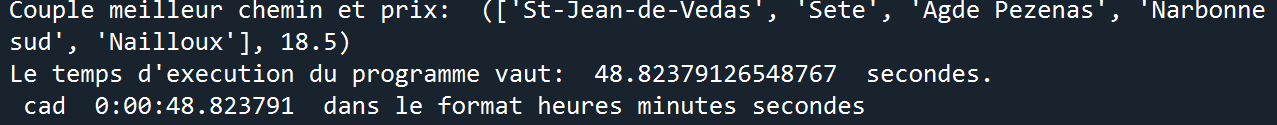
\includegraphics[scale=0.5]{output_exemple.png}
						\caption{Le trajet optimal avec son coût}
					\end{center}
				\end{figure}
			\end{itemize}
		\end{block}
	\end{frame}

	\begin{frame}{Minimisation coût du trajet}
		\tiny
		Par exemple, pour utiliser la fonction \textbf{CreateGraphOfBestPathForPrice}, il suffit d'importer \textbf{Coberny} et d'utiliser la commande suivante:
		\begin{block}{\tiny Exemple d'utilisation}
			\tiny
			Coberny.CreateGraphOfBestPathForPrice( \\
			data, ville\_depart, ville\_arrivee, nbr\_sorties\_max \\
			) \\
			Les arguments de cette fonction sont les même que ceux de la fonction \textbf{FindBestPathForPrice}.
		\end{block}
	
		\begin{block}{\tiny Exemple de sortie obtenue}
			\tiny
			Voici un exemple de ce que retourne la fonction \textbf{CreateGraphOfBestPathForPrice} en prenant les même arguments que ceux utilisés dans la slide précédente.
				\begin{figure}
					\begin{center}
						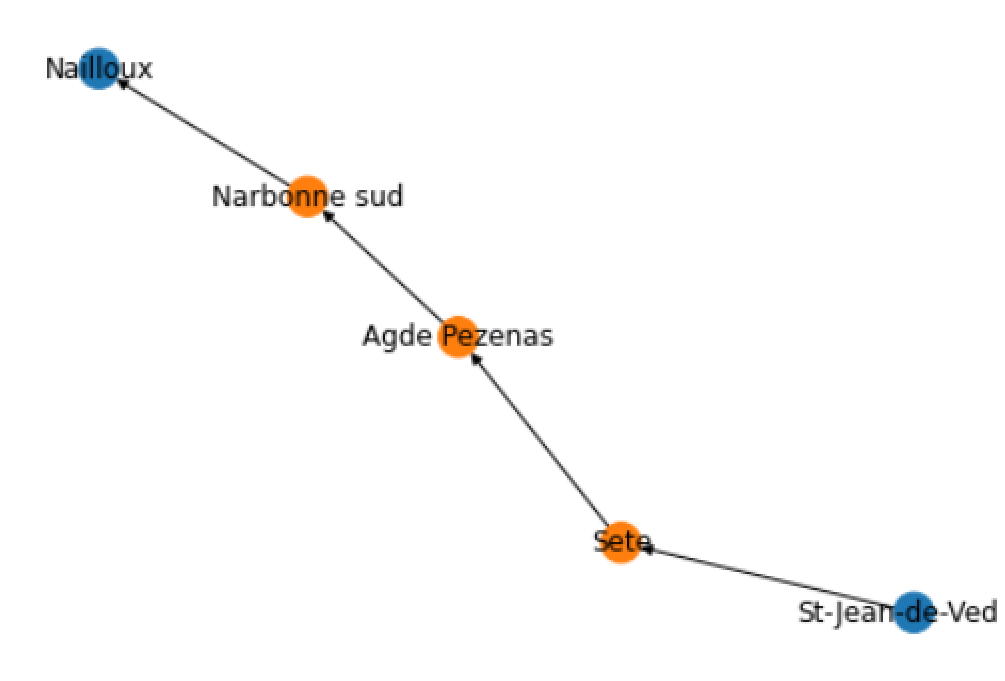
\includegraphics[scale=0.24]{graph_exemple.png}
						\caption{\tiny Graph du trajet optimal}
					\end{center}
				\end{figure}
		\end{block}
	\end{frame}

	\begin{frame}{Minimisation coût du trajet}
		\begin{block}{Utilisation de l'interface utilisateur}
			Nous avons crée une interface utilisateur à  partir du fichier \textbf{best\_price\_pathUI.py}. Ce dernier utilise les fonctions du fichier \textbf{bestPricePathForUI.py}.
			Cette interface va permettre à  l'utilisateur de sélectionner ses données puis de charger les villes de départ. Ensuite, il pourra directement via des menus déroulants, sélectionner la ville de départ, la ville d'arrivée ainsi que le nombre de sorties maximal souhaité (Cela permet d'éviter des erreurs de saisies). Enfin, il pourra exécuter l'algorithme en cliquant sur le bouton "\textit{Trouver le meilleur trajet au meilleur prix}".
		\end{block}
	\end{frame}

	\begin{frame}{Minimisation coût du trajet}
		\scriptsize
		\textbf{Affichage de l'interface utilisateur et exécution de l'algorithme pour le} \textbf{trajet de Sete à  Sigean avec $k = 4$:}
		\begin{figure}
			\begin{center}
				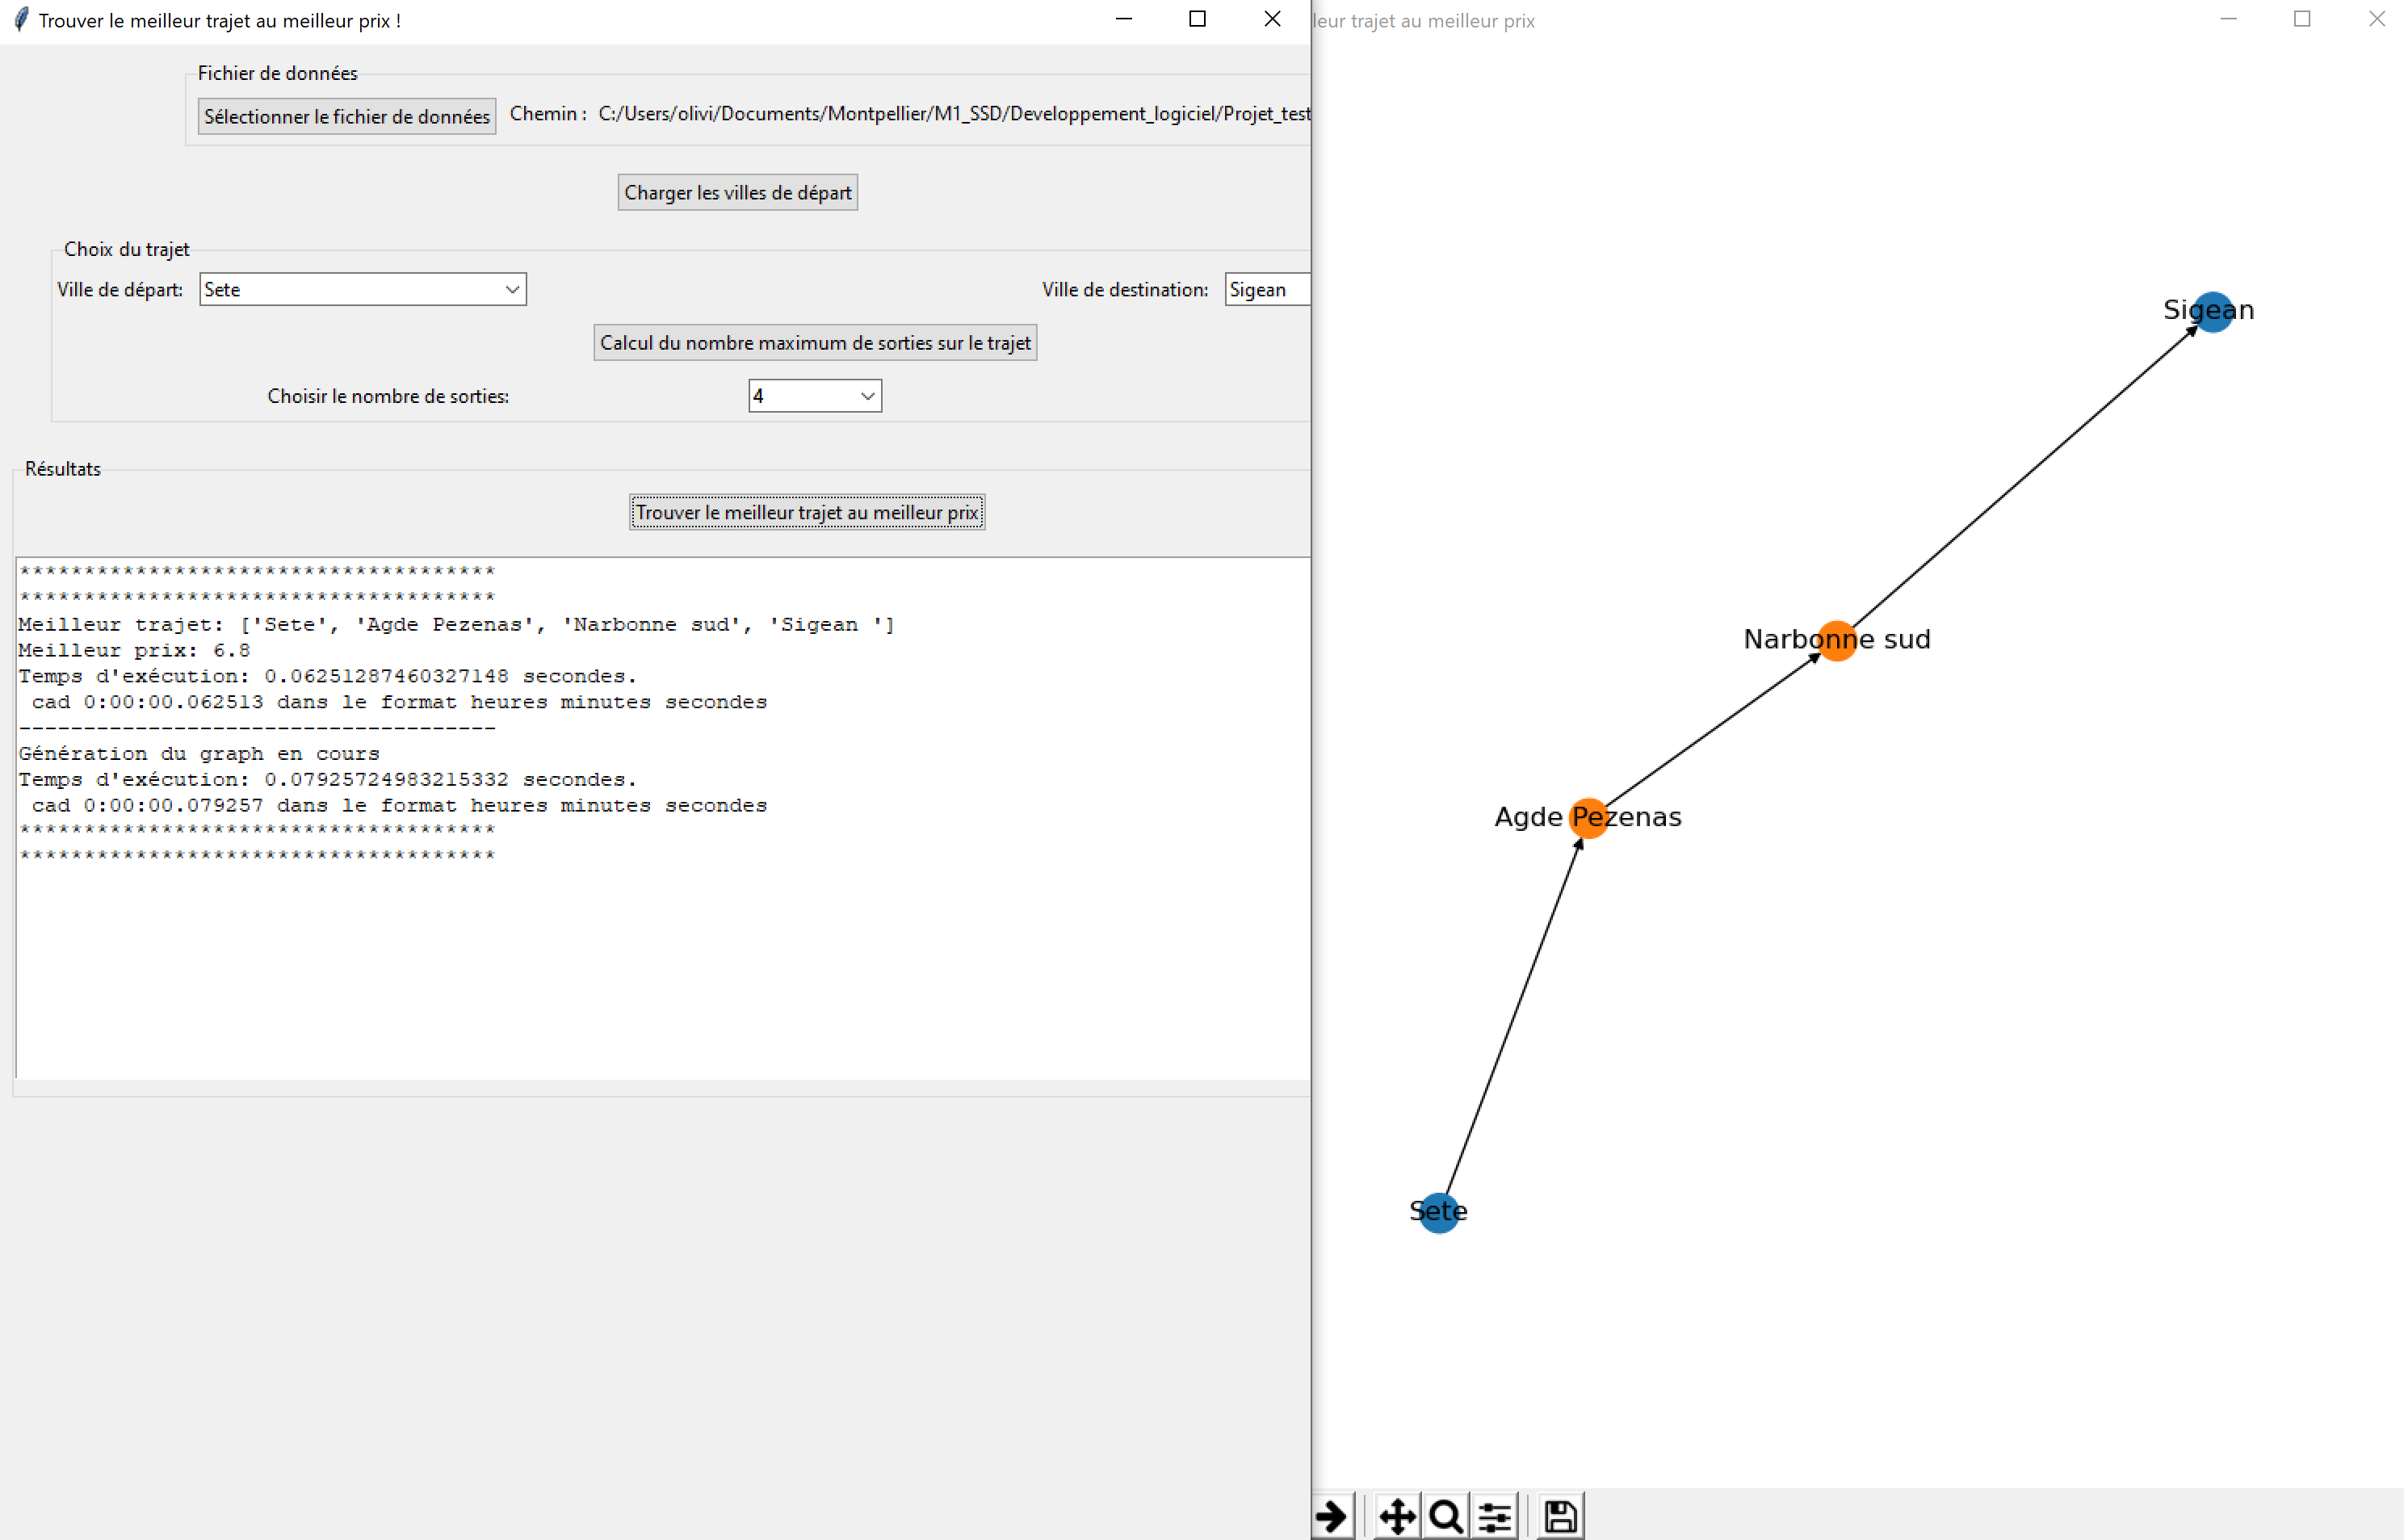
\includegraphics[scale=0.22]{UI.png}
				\caption{\scriptsize Interface utilisateur }
			\end{center}
		\end{figure} 
	\end{frame}


\begin{frame}{}

\includegraphics[width=10cm]{Racoon.jpg}
\end{frame}
\end{document}
